%%=====================================================================
%%  怀化学院本科生毕业论文（设计、创作）LaTeX 模板 —— 主文件
%%
%%  模板名称：怀化学院本科毕业设计 LaTeX 模板
%%  作者：张乐冰 怀化学院 计算机与人工智能学院
%%  版本：V1.1.3  2026.9.10
%%  项目主页： https://github.com/jimmykim84/hhxy-thesis-template 
%%
%%  特别说明：本模板为非官方模板，仅参照本校学位论文格式制作，仅供排版参考；不代表学校官方要求，也不代表示例论文内容正确。如与学校最新官方文件冲突，以学校官方文件为准。
%%
%%  编译方式（必须用 XeLaTeX，编译两遍以生成目录与交叉引用）：
%%      xelatex main.tex
%%      xelatex main.tex
%%
%%  填写位置：本文件"一、论文信息"区；正文写在 chapters/ 下各 .tex 文件。
%%=====================================================================
\documentclass{hhxythesis}

%%=====================================================================
%%  一、论文信息（封面与摘要用到）
%%=====================================================================
\ClassificationNumber{0809}                    % 学科分类号
\ThesisType{本科生毕业设计}                     % 本科生毕业论文 / 毕业设计 / 毕业创作
\WorkType{毕业设计}                             % 诚信声明正文中的称呼
\TitleCN{基于微信小程序的 PMP 刷题系统的实现}
\TitleEN{Implementation of the PMP Answer System Based on the WeChat Mini Program}
\Author{冉\quad 娜}
\StudentID{1406404054}
\College{计算机科学与工程学院}
\Major{网络工程}
\Advisor{杨夷梅}{副教授}                        % 姓名 + 职称
%% 第一指导教师不具备讲师及以上职称时，启用第二指导教师，封面分两行填写：
% \SecondAdvisor{某某}{讲师}
\Duration{2019.06 --- 2020.05}
\SubmitDate{2020 年 5 月 10 日}

%% PDF 文档属性：标题/作者自动取自上方"一、论文信息"，改题或改名时此处无需再动
\makeatletter
\hypersetup{
  pdftitle   = {\hhxy@titlecn},
  pdfauthor  = {\hhxy@author},
  pdfsubject = {怀化学院本科毕业设计},
}
\makeatother

%%=====================================================================
%%  二、正文
%%=====================================================================
\begin{document}

%% ---- 封面（不编页码）------------------------------------------
\makecover

%% ---- 诚信声明（不编页码）--------------------------------------
\makedeclaration

%% ---- 目录（不编页码）------------------------------------------
\makehhxytoc

%% ---- 中英文摘要：页码用罗马数字编排----------------------------
\pagenumbering{Roman}
% %%=====================================================================
%%  中英文摘要与关键词
%%  【规范 6.】中文"摘要""关键词"标示字 4 号黑体居中，内容小 4 号仿宋；
%%            英文"Abstract""Key words"标示字 4 号 Times New Roman 体居中，
%%            内容小 4 号 Times New Roman 体。
%%=====================================================================

%%---------------------------- 中文摘要 -------------------------------
\begin{cnabstract}
本系统主要用于解决传统纸质试卷答题知识点巩固模式以及 PC 端答题系统刷题模式受时间、地点以及费用成本较高的问题。本文实现的 PMP 刷题系统是一款全新的基于微信小程序的知识类小程序，采用微信小程序原生组件搭建基本框架，运用 MVVM 设计模式使用 JavaScript 语言进行编程，实现了快速刷题、查看历史记录、查看排行榜、留言板、随机抽卡片、分享等在线功能。系统汇集了幸运占卜、继续刷题、查看题目解析、查看答题记录、排行榜得分分享等实用功能，方便用户快速了解自己的 PMP 知识储备情况并进行错题回顾。同时，本小程序资源占用率小、运行速度快、界面优雅、操作简洁，能够很好地满足用户的 PMP 刷题需求。
\end{cnabstract}

%%---------------------------- 中文关键词 -----------------------------
\begin{cnkeywords}
微信小程序；PMP；移动端答题
\end{cnkeywords}

%%---------------------------- 英文摘要 -------------------------------
\begin{enabstract}
This system is mainly used to solve the problem that the traditional paper-based
knowledge consolidation mode and the PC-based question-brushing mode are limited
by time, place and high cost. The PMP answer system implemented in this paper is
a new knowledge mini program based on the WeChat Mini Program. It builds the
basic framework with the native components of WeChat Mini Program, and programs
in JavaScript with the MVVM design pattern. The system realizes the online
functions of fast question brushing, history checking, ranking checking, message
board, random card drawing and sharing. It also integrates practical functions
such as lucky divination, continuing to brush questions, viewing item analysis,
viewing answer records and sharing ranking scores, so that users can quickly
understand their PMP knowledge reserve and review the wrong questions. At the
same time, the mini program occupies few resources, runs fast, and has an
elegant interface and simple operation, which can well meet the users' needs of
PMP question brushing.
\end{enabstract}

%%---------------------------- 英文关键词 -----------------------------
\begin{enkeywords}
WeChat Mini Program; PMP; Answer in mobile terminal
\end{enkeywords}
        % 0 摘要

%% ---- 引言/前言起：页码用阿拉伯数字连续编排，至附录--------------
\clearpage
\pagenumbering{arabic}
\mainbody                                % 正文起始：复位为小4仿宋，与摘要一致

%%=====================================================================
%%  1 前言
%%  【规范】一级标题：小 4 号黑体，顶格；正文：小 4 号仿宋，首行缩进 2 字符。
%%=====================================================================
\section{前言}

随着互联网和移动设备信息技术的快速发展，智能移动终端设备得到了极大的普及，人们获取外界信息的习惯也从曾经的报纸、书籍慢慢转变为通过互联网直接获取相关信息。众所周知，学习习惯对于人们来说是需要慢慢培养的，因此伴随着互联网的高速发展，人们从传统的纸质书籍学习拓展到了如今的线上学习，这是一个伟大的转变。相较于传统的学习方式，线上学习具有以下优势。

首先，不受学习时间和空间的限制。许多上班族都会选择网上学习的方式学习一些跟自己职业生涯相关的知识，特别是对于部分职场新人，由于个人工作能力的欠缺、工作经验的不足，往往会通过线上学习的方式获取需要的专业知识。对于大部分上班族来说，白天需要专心于公司的工作，而晚上又可能需要处理各种各样的个人问题或者家庭问题，导致没有办法挤出大量的时间去实体班系统化地学习。但是，线上学习则可以方便地配合个人的时间与地点，只要有网络和移动终端设备就可以随时随地利用个人碎片化的时间快速开始学习。

其次，线上学习费用更低。自 2005 年以来，各种类型的线上教育平台如雨后春笋般涌现，其发展如此迅猛的原因之一就是费用和资源得到了大量节省。相对于传统教育的模式，线上教育节省了住宿、教师、教室、资料等大量资源，据不完全统计，线上学习大致花费仅相当于传统现场学习费用的 30\%---50\%\footnote{该比例引自在线教育行业公开调研数据，不同机构的统计口径存在差异。}，却可以达到相差无几的学习效果\cite{bib:moodle}。

最后，更强的可重复性与个性化学习。线上学习可以根据个人学习需求和学习进度反复学习，重复未理解的部分，以便更好地掌握所学内容并充分巩固学习效果，避免在传统课堂学习中容易出现的"学过就忘"的问题。同时，线上学习能够较好地实现个性化学习，人们可以根据个人的时间安排，依照个人的需求、文化背景、学习习惯来选择学习内容，有效地增强学习的针对性和提高学习效率。

在移动终端上，一个 APP 应用程序需要 Android 和 iOS 两套技术代码，应用程序的上传步骤繁琐，开发周期较长。同时，一个优秀的 APP 应用的研发与推广，不仅需要配备优秀的产品经理、市场运营人员，还需要高额的推广成本。此外，部分 APP 界面操作复杂，占用较多手机内存，需要用户授予诸多权限等因素，造成许多用户不愿意轻易下载 APP 应用程序。

微信小程序不需要用户安装，即开即用，节省了许多用户流量和安装时间。相较于原生 APP，小程序不但在用户使用体验感上差别不大，而且在开发成本、获客成本、下载便捷程度以及轻应用方面具有更大的优势。微信小程序与第三方应用不同，无需频繁地跳出微信再重新回到微信，减少了用户许多重复性的操作，提升了用户体验。微信小程序依附于微信生态系统的环境下，因而后期的技术维护比原生 APP 更加容易。截止到 2016 年第二季度，微信已经覆盖国内 94\% 以上的智能移动终端，月活跃用户量达到 8 亿以上，用户覆盖超过 200 个国家、20 种语言，微信公众账号的总数超过 800 万个，移动应用程序的对接数量超过 85000 个\cite{bib:xiong}。

这次我们所设计的课题系统，正是移动终端设备社交平台与社会生活之间紧密关系的体现。随着微信的迅猛发展，微信逐渐成为现代人生活中一个重要的组成部分，它对用户信息的获取、电子商务、生活服务、即时交流等许多方面产生了深刻的影响。微信小程序依托微信庞大的用户流量，以一种全新的方式连接用户与服务。本论文以增强移动端用户 PMP 考证刷题的便捷性和实时性为目的，设计并实现了基于微信小程序的 PMP 刷题系统。
         % 1 前言
%%=====================================================================
%%  2 微信小程序开发介绍
%%=====================================================================
\section{微信小程序开发介绍}

\subsection{微信小程序系统架构}

微信小程序采用了视图层与逻辑层分离的双线程架构，其结构层次如图 \ref{fig:architecture} 所示\cite{bib:lei}。

\begin{figure}[htbp]
  \centering
  \figurenote{图中箭头表示数据与事件的传递方向。}
  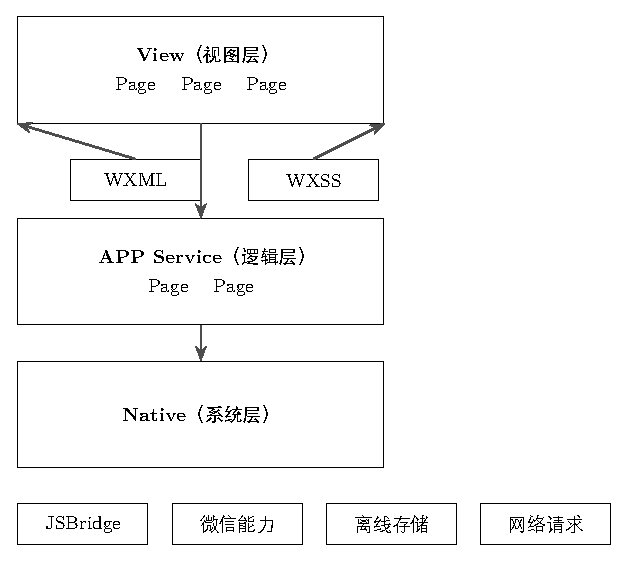
\includegraphics[width=0.72\textwidth]{figures/fig-architecture.pdf}
  \caption{刷题系统结构层次图}
  \label{fig:architecture}
\end{figure}

View（视图层）主要由 WXML、WXS 与 WXSS 组合编写，通过原生热布局的方式由组件来进行展示，主要用于将逻辑层的数据渲染到视图层，同时将视图层的事件传递给逻辑层。View 的 Component 以 Web Component 为标准，通过 Polymer 框架实现。Native 组件层在 Web View 层之上，由 View 的 Native Component 实现的组件有 \texttt{canvas}、\texttt{video}、\texttt{map}、\texttt{textarea} 等。

WXML（WeiXin Markup Language）是专门为微信小程序框架设计的标签语言，采用将基础组件和事件系统结合的方式构建页面的结构。WXML 类似于 HTML，是微信开发的一种标记语言，仅支持使用其指定的对应组件，例如 View、Block、Button、View-Scroll、Image、Text、Navigator 等。WXML 还具有数据绑定、列表渲染、条件渲染、模板、事件和引入等功能。其中，数据绑定使用双大括号进行双向绑定；列表渲染通过 \texttt{wx:for} 引用在 JavaScript 中定义的数组变量；条件渲染使用 \texttt{wx:if}、\texttt{wx:elif}、\texttt{wx:else} 判断。

WXS（WeiXin Script）是专门用于微信小程序的一套脚本语言，与 WXML 结合使用构建页面结构。WXS 能够在所有版本的微信小程序中运行，不依赖于当前运行的基础库版本。它拥有自己的语法规则，与 JavaScript 不一致，属于不同的编程语言。由于存在运行环境的差异，小程序内的 WXS 在 iOS 设备上运行会比 JavaScript 代码快 2 到 20 倍，在 Android 设备上二者运行效率相差无几。

WXSS（WeiXin Style Sheets）是专门为小程序设计的一套样式语言，用于描述页面结构中组件的显示方式，例如字体大小、背景颜色、定位方式等。为了便于前端开发者开发微信小程序，WXSS 具有 CSS 的大部分特性，并对 CSS 进行了扩充和修改\cite{bib:css,bib:html5}。与 CSS 相比，其扩展特性主要包括尺寸单位和样式导入两项。小程序使用 rpx（Responsive Pixel）作为尺寸单位，它是一个根据屏幕宽度自适应的尺寸单位，规定屏幕宽度为 750\,rpx。这意味着无论移动设备屏幕有多大，宽度都是 750 个 rpx；这是一个绝对大小，但是每个 rpx 的具体大小由移动终端的具体尺寸来决定。

APP Service（逻辑层）由 JavaScript 实现编写与封装，主要用于将逻辑层的数据进行处理后渲染到视图层，并对视图层用户行为的事件进行反馈。小程序各个页面中的网络通信、应用生命周期管理、数据管理以及页面路由都是由 App Service 实现的。由于页面是在 JsCore 中运行脚本逻辑，而 JsCore 是没有窗口对象的环境，所以小程序不能在脚本中使用 Document、Window 对象，也不能直接操作 DOM 节点和组件。因为 Zepto、jQuery 中使用了 Document、Window 等对象，所以它们在小程序中都无法被使用\cite{bib:jquery}。

Native（系统层）通过对微信客户端所提供的网络数据通信、文件系统管理、数据安全任务管理等基础功能进行封装，对上层提供一整套非常完整的 JavaScript API。由于小程序是通过 JSBridge 实现对底层原生 API 接口的调用，而 JSBridge 是架起上层开发与 Native（系统层）的桥梁，因此小程序可通过 API 直接使用原生的功能。

\subsection{微信小程序开发语言 JavaScript}

JavaScript 是一种通过解释执行的高级编程语言，是一门基于原型、函数先行、动态类型、面向对象的解释型语言。它已由 ECMA（欧洲电脑制造商协会）通过 ECMAScript 实现了语言的标准化。世界五大主流浏览器都已支持使用 JavaScript，绝大多数的网站都使用 JavaScript 实现动态交互\cite{bib:zakas}。JavaScript 支持面向对象编程、命令式编程以及函数式编程，它提供一系列的语法来控制节点、对象、日期、文本、数组以及正则表达式等。

一般情况下，完整的 JavaScript 包括以下几个部分：ECMAScript，用于描述该语言的语法和基本对象；文档对象模型（DOM），用于描述处理网页内容的方法和接口；浏览器对象模型（BOM），用于描述与浏览器进行交互的方法和接口。JavaScript 主要用于为 HTML 页面添加交互行为，可以直接嵌入 HTML 页面，单独引入的外部 JS 文件更有利于行为和结构的分离\cite{bib:ruan}。

与服务器端脚本语言不同，JavaScript 不需要服务器的支持，它被当作客户端的脚本语言在浏览器上运行。随着 HTML5、CSS3 语言标准的推行以及 JavaScript 事件驱动和异步 I/O 等特性的应用，它还可用于网络游戏、移动应用程序的开发以及在服务器端的网络环境运行，如 Node.js。

\subsection{微信 Web 开发工具}

微信 Web 开发者工具是由微信官方推出的专门用于帮助开发者更简单和高效地开发、调试微信小程序以及微信公众号的开发工具。它主要通过模拟微信客户端的表现，使开发者可以便捷地在 Mac 或者 PC 上进行开发和调试工作。它集成了小程序调试和公众号网页调试两种开发模式。使用小程序调试，开发者可以实现小程序的部分 API 的调用、代码查看和编辑、页面的开发调试、远程调试、小程序预览和发布等功能。

开发者可以直接在微信开发者工具中进行项目编辑、调试、预览、上传、编译、切换项目运行场景、模拟器尺寸以及切换模拟网络环境等。小程序在模拟器和真机上的运行效果基本相同，只是模拟器没有拨打电话、重力感应、发送短信、蓝牙等功能。但是由于运行环境的差异，部分 API 在开发者工具上的调试结果与真机的调试结果并不完全一致，例如 \texttt{wx.getUserInfo}、\texttt{wx.chooseInvoiceTitle} 等。因此，开发者如果需要进行调试，可以使用微信开发者工具的远程调试功能，并以真机调试为准。
     % 2 微信小程序开发介绍
%%=====================================================================
%%  3 微信小程序开发需求设计
%%=====================================================================
\section{微信小程序开发需求设计}

\subsection{用户需求分析}

PMP 刷题系统的用户对象是所有使用微信且有 PMP 刷题需求的用户，用户需求主要有以下几个方面：

\begin{enumerate}
  \item 用户可以选择每次答题的数量和章节；
  \item 用户可以进行在线快速答题；
  \item 用户答题完毕后可以查看答案解析；
  \item 用户可以查看历史记录，查看已做过题目的答案解析；
  \item 用户可将小程序发送至微信好友或微信群；
  \item 用户可以查看不同群的好友答题得分排名；
  \item 用户遇到问题可以进行留言反馈；
  \item 用户可以查看距离下一次考试的天数倒计时；
  \item 用户每日可进行一次运势占卜，占卜的结果可分享或保存在本地。
\end{enumerate}

\subsection{功能需求分析}

以用户需求为出发点，结合微信小程序开发的基本要求，本 PMP 刷题系统主要实现在线快速刷题、查看历史记录、查看群排名、幸运占卜、咨询反馈、分享等在线功能。具体要求如下。

快速刷题：用户能够选择每次答题数目和答题章节，并且答题完毕后才显示"提交答题"按钮。提交答卷后显示本次答题正确率，用户可以选择继续刷题或者查看本次答题解析。

查看历史记录：可以查看已答过的试卷信息，以红绿两色区分正确与否。点击对应的答题记录可以查看对应的题目解析。

查看群排行榜：可以查看已经分享过的微信群内的群成员答题总分以及群排名，并且不同的微信群中的排名可能不同。

咨询反馈：用户可以将在小程序使用过程中的问题，通过留言板反馈给后台。反馈的信息中除用户描述的问题，还会包含用户的设备信息。

幸运占卜：用户每日做满 20 题，可以进行一次幸运抽牌。包含洗牌、蜡烛移动、眨眼、音效播放等动画效果。

分享：用户可以将当日抽签的卡片、答题群排行榜得分分享至微信群，其他微信用户可以从分享的卡片进入小程序。同时，用户可以将当日抽取的卡片保存至手机相册，并可主动分享图片至微信朋友圈。
     % 3 微信小程序开发需求设计
%%=====================================================================
%%  4 项目主要技术实现介绍
%%=====================================================================
\section{项目主要技术实现介绍}

项目开发中需要用到多种设计模式、JSON 解析、界面设计等技术，以下对各项技术做简单介绍。

\subsection{PMP 刷题系统使用的几种设计模式}

（1）MVVM 模式

MVVM（Model-View-View Model）是一种软件架构模式，它有利于将图形用户界面的开发与后端业务逻辑以及数据模型的开发进行分离。它实现了关注点的分离，解决代码紧密耦合、易变动、结构性不强导致难以长期维护的问题，最终达到提高用户体验的目的\cite{bib:zeng}。MVVM 模式将应用程序分成以下几个主要部分，其原理如图 \ref{fig:mvvm} 所示。

\begin{figure}[htbp]
  \centering
  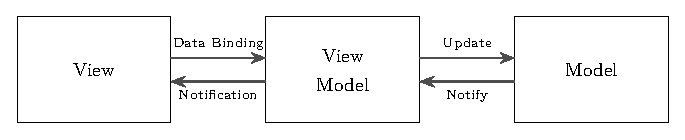
\includegraphics[width=0.78\textwidth]{figures/fig-mvvm.pdf}
  \caption{MVVM 原理图}
  \label{fig:mvvm}
\end{figure}

Model（模型）是指任何一个领域模型，代表一个面向对象的方法或者以数据为中心的数据访问层。它主要用于将应用程序中与业务逻辑相关的数据和该数据的处理方式进行封装，能够直接访问数据，例如对后台数据库的访问。Model 不依赖 View 和 View Model，即模型不关心被如何操作，也不包含任何用户界面的相关业务逻辑。

View（视图）是应用程序中用户可见的界面。视图对象不但了解如何将自己绘制出来，而且可能会对用户的操作做出相应的响应。视图对象的目的是显示来自应用程序模型对象的数据，并使该数据能够被编辑。尽管如此，通常情况下在 MVVM 应用程序中，视图对象与模型对象是分离的。

View Model（视图模型）是暴露公共属性与命令的视图的抽象，作为 View 与 Model 之间的桥梁，通过双向数据绑定把 View 层和 Model 层进行连接。开发者只需要关注业务逻辑的处理，因为 View 和 Model 之间的同步工作完全是自动的，无需人为干涉，无需手动操作 DOM 结点，也无需关注数据状态的同步问题。

（2）代理模式

代理模式（Proxy）主要用于为其他对象提供一种代理进而控制对这个对象的访问。代理模式使得代理对象能够控制具体对象的引用。代理几乎能够是任何对象：资源、文件、内存中的对象，或者是一些无法复制的东西。代理模式主要可以分为虚拟代理、缓存代理和用高阶函数动态创建代理三种。在 JavaScript 开发中最常用的是虚拟代理和缓存代理。

（3）观察者模式

观察者模式一般作为 Model 层对 View Model 的通知方式，不在意哪一层接收，只需要负责发布信息。它定义了一种一对多的关系，实现了多个观察者对象同时对某一个主体对象的监听，只要这个主体对象的状态发生任何变化就会通知所有的观察者对象，使得观察者们能够自动更新。

（4）单例模式

单例就是保证每次只有一个实例，实现方法一般是先判断实例是否存在，如果存在，则直接返回；如果不存在，则创建后再返回，从而确保只有一个实例对象。在 JavaScript 中，单例从全局命名空间内提供一个唯一的访问点来访问该对象，被作为一个命名空间提供者。

\subsection{JSON 技术的使用}

JSON（JavaScript Object Notation）是一种轻量级的数据交换格式。它是基于 ECMAScript 的一种完全独立的文本格式，采用完全独立于任何编程语言的文本格式进行数据的存储，主要用来传输由序列化的值或属性值组成的数据对象。同时，JSON 因其简洁和清晰的结构层次成为目前较为理想的数据交换语言。它的官方 MIME 类型是 \texttt{application/json}，文件扩展名是 \texttt{.json}。

JSON 主要由两种结构构建：第一种是"名称/值"对的集合，以左花括号开始、以右花括号结束，每一个"名称"后有一个冒号，多个"名称/值"对之间使用逗号作为分隔符；第二种是值的有序列表，一个数组以左中括号开始、以右中括号结束，多个值之间使用逗号作为分隔符。其中，值可以是被双引号包裹的数字、字符串、布尔值、空值、数组或者对象，这些结构都可以互相嵌套。

\subsection{PMP 刷题系统界面的实现}

小程序中的界面主要通过两部分实现。首先完成界面的布局，然后通过网络请求得到数据并将数据填充在相对应的界面。

\subsubsection{典型界面布局}

界面主要都是通过以下部分来实现的。通过在 \texttt{app.json} 或者 \texttt{page.json} 文件中对小程序进行全局配置，可以决定窗口表现形式、页面的文件路径、多 tab 的设置、网络请求超时时间的设置等。通过 \texttt{pages} 指定小程序由哪些页面组成，通过 \texttt{window} 设置导航条的背景颜色、导航栏的标题、状态栏、窗口的背景色等。在 \texttt{.wxml} 文件中使用微信小程序封装的指定组件开发页面结构，在 \texttt{.wxss} 文件中设置页面结构样式，在 \texttt{.js} 文件中实现界面逻辑以及生命周期函数的合理使用。其结构如图 \ref{fig:homepage} 所示。

\begin{figure}[htbp]
  \centering
  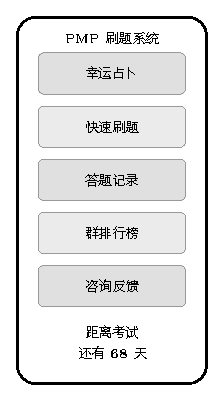
\includegraphics[width=0.30\textwidth]{figures/fig-homepage.pdf}
  \caption{刷题系统首页效果图}
  \label{fig:homepage}
\end{figure}

\subsubsection{数据填充}

首先，通过 GET 或者 POST 请求方式访问服务端的指定接口，获取相关的数据信息。其次，通过对服务端返回的数据进行 JSON 解析以及数据筛选，得到所需数据。最后，将不同接口的数据信息按照界面的布局渲染在相对应的组件上面，从而实现界面的数据填充。
      % 4 项目主要技术实现介绍
%%=====================================================================
%%  5 系统模块设计与实现
%%=====================================================================
\section{系统模块设计与实现}

PMP 刷题系统的模块划分如图 \ref{fig:flowchart} 所示。

\begin{figure}[htbp]
  \centering
  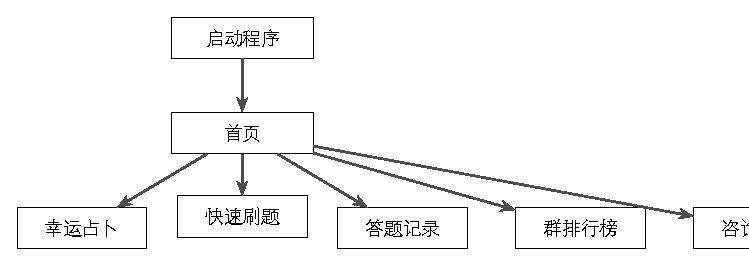
\includegraphics[width=0.80\textwidth]{figures/fig-flowchart.pdf}
  \caption{刷题系统模块流程图}
  \label{fig:flowchart}
\end{figure}

各模块的主要职责如下。

启动程序：进入微信小程序，程序自然启动。进入小程序后，主界面有 5 个模块，分别是幸运占卜、快速刷题、历史记录、群排行榜、咨询反馈。

首页：是整个小程序的门面，汇集五大模块。一般情况下，每次进入小程序最先进入首页。用户在首页可查看小程序的所有功能，从而进行相应的操作。同时，在幸运占卜模块右侧显示当前距离下一次 PMP 考试的天数。

幸运占卜：用户每次答题数满 20 题，可进行一次占卜。在这里用户可以抽取当日的幸运卡片，并将卡片分享至微信群或者将卡片保存至本地相册。

快速刷题：用户可以自己选择答题数量和答题章节进行快速刷题，用户答题完毕提交试卷后可自行选择继续答题还是查看答案解析。

群排行榜：用户可以将个人答题的得分分享至微信群，以及查看对应微信群中使用该小程序的用户的群排行榜得分情况。

答题记录：用户可以查看以往的答题记录，并且查看当时的题目解析。

咨询反馈：用户在使用过程中遇到问题，可以通过此模块进行留言反馈。

在功能实现方面，由于微信小程序 API 嵌套使用会导致代码过于繁琐冗长，且网络请求是异步的，而系统除咨询反馈以外的模块都需要检查登录状态再进行网络请求，因此本系统使用 Promise 和 Proxy 对网络请求和微信小程序的 API 进行了二次模块化封装，关键代码如下：

\begin{lstlisting}[style=js]
/* 对网络请求和自定义空 Promise 的封装 */
let services = {
  taskSequence: () => new Promise((resolve, reject) => { resolve(); }),
  httpClientPost: (url, data) => new Promise((resolve, reject) => {
    wx.request({
      url: url, data: data, method: 'POST',
      header: { 'Content-Type': 'application/json',
                'token': wx.getStorageSync('token') || '' },
      success: (res) => { resolve(res); },
      fail:    (res) => { reject(res);  },
    });
  }),
};

/* 对微信小程序的 API 通过 Proxy 进行二次封装 */
let wsAPI = new Proxy(services, {
  get: function (target, property) {
    if (property in target) { return target[property]; }
    else if (property in wx) {
      return (obj) => new Promise((resolve, reject) => {
        obj = obj || {};
        obj.success = (...args) => { resolve(...args); };
        obj.fail    = (...args) => { reject(...args);  };
        wx[property](obj);
      });
    }
  }
});
\end{lstlisting}

\subsection{首页界面设计与实现}

首页界面的布局主要采用了 MVVM 模式，建立数据模型，在 View 里面进行组件内容的显示，通过双向数据绑定来实现数据之间的交互。从主页跳转到其他页面通过调用 \texttt{wx.navigateTo} 或者 Navigator 组件实现，由于微信小程序的标签与 HTML 标签存在差异，所以无法通过 a 标签进行页面跳转。由于小程序的 Image 组件不支持使用本地图片，所以首页各模块的背景图片使用的是网络地址。

项目启动后，立即发出首页数据的网络请求，将请求获取到的数据解析并渲染到页面上。同时，对用户是否已经对小程序授权以及登录进行判断，若用户未授权，则弹出微信小程序系统授权框，引导用户授权使用小程序。

\subsection{快速刷题界面设计与实现}

快速刷题这个模块是答题系统的主要功能模块。具体实现：进入答题页面时，判断用户是否授权登录，若用户未授权则引导用户授权。然后将用户在首页选择的答题数量和答题章节通过网络请求发送给后台，从而获取到题目信息，并通过数据双向绑定的方式渲染答题界面。代码设计主要采用 MVVM 模式，通过代理模式请求网络通信和微信的 API，从而进行数据交互；通过封装的自定义模块显示 toast、modal 以及 loading；通过设置开关，避免用户多次点击造成数据的多次请求、渲染等问题。

用户提交试卷后，本次答题信息将通过网络请求传递给后台，后台接收参数进行一系列处理，将答案解析反馈回前端，用户可以选择继续答题或者查看答案解析。本次答题的正确率按式（\ref{equ:accuracy}）计算：

\begin{equation}
  P = \frac{N_{\mathrm{right}}}{N_{\mathrm{total}}} \times 100\%
  \label{equ:accuracy}
\end{equation}

式中：$P$ 为本次答题正确率；$N_{\mathrm{right}}$ 为答对题数；$N_{\mathrm{total}}$ 为本次答题总题数。

\subsection{群排行榜界面设计与实现}

群排行榜模块主要用于显示用户在不同的微信群中的排名情况。首次进入微信小程序的用户将小程序分享至一个或多个微信群中，才会获取到相对应的群组信息以及群成员排名信息。非首次进入小程序的用户，进入群组页面后会通过网络请求获取群组信息，再通过数据双向绑定渲染页面。

\subsection{答题记录界面设计与实现}

答题记录模块主要用于显示以往的答题记录，显示以往答题的正确率以及对应的试卷答案解析。这个界面可以采用上拉刷新加载更多，每一次上拉刷新都要请求一次服务器。上拉刷新实现的原理：每次上拉的时候请求服务器，服务器都会返回最新的第一页的数据，然后再把数据源添加到原数据数组的尾部，接着重新渲染当前页面，从而实现上拉刷新。

\subsection{咨询反馈界面设计与实现}

咨询反馈模块主要用于用户反馈小程序使用过程中遇到的问题，此模块不需要用户登录。用户提交留言后，会将用户反馈的信息以及用户机型等相关信息通过网络请求反馈给后台。

\subsection{幸运占卜界面设计与实现}

幸运占卜模块主要用于用户每日做题满 20 题后抽取当日幸运卡片。进入页面时会判断用户是否授权，若未授权则引导用户授权登录。若当日用户未做满 20 题，则显示眼睛特效——眼睛周围的图片根据重力感应可进行移动，点击蜡烛和眼睛都会播放对应的音效。用户在进入页面时会通过网络请求获取到本次抽签卡片的相关信息，并在用户抽签结束后渲染到卡片页面。用户可将抽取的卡片分享至微信群或将卡片保存在本地\cite{bib:qie}。
       % 5 系统模块设计与实现
%%=====================================================================
%%  6 测试
%%=====================================================================
\section{测试}

\subsection{测试目的}

软件测试的主要目的是测试小程序的界面实现与设计的效果是否吻合、程序运行效果是否良好、功能是否实现。通过测试及时发现潜在的问题，立即修正，使所有的功能模块能够达到预期标准，提升用户体验。

\subsection{测试环境}

进行测试的手机为小米 6，其 CPU 架构为高通骁龙 835 八核处理器，CPU 频率为 2.45\,GHz，RAM 容量为 6\,GB，ROM 容量为 64\,GB，手机主屏尺寸为 5.15 英寸，屏幕分辨率为 $1920 \times 1080$ 像素，手机的摄像头分辨率为 1200 万像素，手机的操作系统使用的是 Android 8.0。

\subsection{测试结果}

对系统的主要页面和功能点的测试用例如下。

（1）授权登录的测试用例如表 \ref{tab:test-login} 所示。

\begin{table}[htbp]
  \centering
  \caption{授权登录测试用例}
  \label{tab:test-login}
  \begin{tabular}{|c|p{9.6cm}|}
    \hline
    用例名称 & 授权登录 \\
    \hline
    目\quad 的 & 测试小程序获取用户信息授权的功能 \\
    \hline
    前\quad 提 & 用户首次进入小程序 \\
    \hline
    测试流程 & 用户第一次进入小程序，弹出系统授权框，点击"允许" \\
    \hline
    预期结果 & 成功获取用户头像、昵称，并写入后台用户表 \\
    \hline
    实际结果 & 实际结果与预期结果一致 \\
    \hline
  \end{tabular}
\end{table}

（2）快速刷题的测试用例如表 \ref{tab:test-brush} 所示。

\begin{table}[htbp]
  \centering
  \caption{快速刷题测试用例}
  \label{tab:test-brush}
  \begin{tabular}{|c|p{9.6cm}|}
    \hline
    用例名称 & 快速刷题 \\
    \hline
    目\quad 的 & 测试快速刷题模块能否正常出题与判分 \\
    \hline
    前\quad 提 & 用户已授权登录 \\
    \hline
    测试流程 & 用户在首页选择答题数量与章节，进入答题页并作答，提交试卷 \\
    \hline
    预期结果 & 按所选数量与章节正确出题，提交后显示正确率，可查看答案解析 \\
    \hline
    实际结果 & 实际结果与预期结果一致 \\
    \hline
  \end{tabular}
\end{table}

（3）群排行榜的测试用例如表 \ref{tab:test-rank} 所示。

\begin{table}[htbp]
  \centering
  \caption{群排行榜测试用例}
  \label{tab:test-rank}
  \begin{tabular}{|c|p{9.6cm}|}
    \hline
    用例名称 & 群排行榜 \\
    \hline
    目\quad 的 & 测试分享后能否正确获取群成员排名信息 \\
    \hline
    前\quad 提 & 用户已将小程序分享至至少一个微信群 \\
    \hline
    测试流程 & 用户从排行榜页面分享卡片，其他群成员通过该卡片进入小程序 \\
    \hline
    预期结果 & 通过 shareticket 获取对应群成员列表，并正确显示得分排名 \\
    \hline
    实际结果 & 实际结果与预期结果一致 \\
    \hline
  \end{tabular}
\end{table}

测试结果主要显示小程序的使用性能情况。通过测试能找到小程序在手机上的性能使用情况，从而让更多的用户接受并使用本刷题系统。测试内容主要包括各页面 CPU 占比、加载时间、内存占比等性能\cite{bib:souders}，测试结果如图 \ref{fig:perf} 所示。

\begin{figure}[htbp]
  \centering
  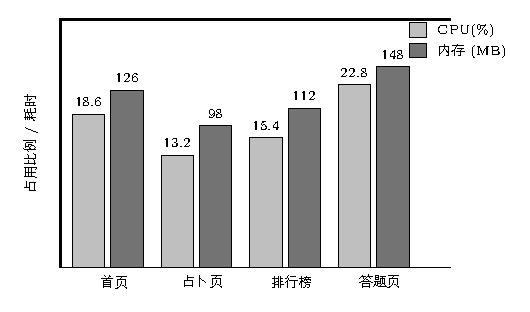
\includegraphics[width=0.86\textwidth]{figures/fig-perf.pdf}
  \caption{各页面性能测试图}
  \label{fig:perf}
\end{figure}

由测试结果可以看出，四个主要页面的 CPU 占用率均低于 25\%，内存占用均低于 150\,MB，页面平均加载时间在 1\,s 以内，各项性能指标均满足轻应用类小程序的上线要求。
            % 6 测试
%%=====================================================================
%%  7 总结
%%=====================================================================
\section{总结}

本系统具有快速刷题、查看群排行榜、查看历史答题记录、在线咨询、幸运占卜等功能。这个项目的开发难度主要有两点。第一点，幸运占卜中的特效比较复杂、不易控制，蜡烛的点击和移动特效、眼睛的眨眼特效、背景根据重力移动的特效、抽卡动画等全部集中在一个页面中，因此对于动画的控制需要格外注意。第二点，异步操作的链式执行。因为网络请求一般是异步的，所以在一些页面中存在多个请求时可能会造成页面操作的执行顺序不对。最终采用 Promise 封装和 Callback 回调函数的方式进行解决，并对常用请求进行了封装。

通过本次毕业设计，系统地掌握了微信小程序双线程架构的原理、WXML 与 WXSS 的编写方法以及原生 API 的调用方式，同时也深入理解了 MVVM 模式在前端工程中的落地方式。后续可以在题库的智能推荐、错题本的个性化复习提醒等方面继续完善\cite{bib:wang2021}。后续可借鉴面向在线学习的个性化练习推荐方法\cite{bib:zhang2020}，并持续跟进微信小程序官方开发文档\cite{bib:wechatdoc}中的接口更新，以进一步提升用户的学习效率。
         % 7 总结

%%=====================================================================
%%  参考文献
%%  采用 BibTeX 管理：文献数据库在 refs.bib（项目根目录），
%%  著录样式由 gbt7714-2005.bst（项目根目录，已随模板附带，无需安装）控制，
%%  符合 GB/T 7714-2005（顺序编码制：[1] 上标、编号按引用先后）。
%%
%%  本文件只需两行，正文用 \cite{引用键} 交叉引用即可：
%%    \bibliographystyle{gbt7714-2005}   % 著录格式
%%    \bibliography{refs}                % 文献数据库 refs.bib
%%
%%  编译顺序（关键，比纯两遍多了一步 bibtex）：
%%    xelatex main.tex
%%    bibtex  main
%%    xelatex main.tex
%%    xelatex main.tex
%%
%%  注意：标题“参考文献”、5 号仿宋、左顶格 [1] 等版式由 hhxythesis.cls
%%  的 thebibliography 环境统一控制，此处无需再写。
%%=====================================================================

\bibliographystyle{gbt7714-2005}
\bibliography{refs}
       % 参考文献
%%=====================================================================
%%  致谢
%%  【规范】致谢（小 4 号黑体居中，另起一页），正文小 4 号仿宋。
%%=====================================================================

\begin{acknowledgement}
在四年的大学生涯即将结束之际，我衷心地感谢这四年来每一位关心我、帮助我的老师和同学。本次毕业设计与论文的撰写过程中，从材料收集、作品的设计、论文选题、撰写开题报告，到最后的正文撰写，杨夷梅老师给予了我悉心的指导和指导性的意见。杨老师高情商的为人处世、严谨的教学精神以及精益求精的工作作风，让我在完成毕业设计和论文过程中收益良多。在本次论文编写过程中，在杨老师无私的指导和帮助下，我解决了一个又一个的难题。因为杨老师不断指出论文中存在的问题并提出建设性的意见，我的论文才能更加完善。在此向杨老师致以诚挚的谢意和崇高的敬意。

此外，我还想衷心地感谢我的大学室友们。感谢她们在毕业论文修改期间督促我更改论文，积极地帮我修改论文格式和排版；感谢她们四年来的关心与陪伴；感谢她们在我遇到人生重大挫折的时候给我支持与鼓励，在我陷入生活低谷的时候给我希望与关怀。

最后，感谢我生活与学习了四年的母校——怀化学院，感谢母校给了我一个优质的学习平台，让我不断吸取新的知识，充实自己，提升自己。
\end{acknowledgement}
 % 致谢
%%=====================================================================
%%  附录
%%  【规范】附录：（另起一页，小 4 号黑体，顶格）；附录中的公式编号为（A1）。
%%=====================================================================

\begin{theappendix}

本附录给出系统实现过程中的部分核心代码，供评阅与复现参考。

\subsection*{A1\quad 首页视图层结构}

\begin{lstlisting}[style=xml, caption={首页视图层 index.wxml}]
<view class="container" style='align-items: center;'>
  <view class='top_notice' wx:if="{{notAuthorized}}">
    <text>小程序需要您的授权才能正常使用</text>
    <button bindtap='onOpenSetting'>去授权</button>
  </view>
  <view class='index_card_img' bindtap='toPunchcardPage'
        style="background-image:url(https://xxx.com/card.png);">
  </view>
  <view class='index_text_bg'>
    <text class='index_title'>幸运占卜</text>
    <text class='index_subtitle'>每日需刷满20题可进行一次占卜</text>
  </view>
  <view class='countDown'>
    <image src='/images/punchcard/{{day.left}}.png' class='l'></image>
    <image src='/images/punchcard/{{day.right}}.png' class='r'></image>
  </view>
</view>
\end{lstlisting}

\subsection*{A2\quad 抽卡动画处理逻辑}

\begin{lstlisting}[style=js, caption={洗牌动画 onShuffleEvent}]
/* 洗牌 */
onShuffleEvent: function (cb) {
  shuffleCount++;
  this.innerAudioContext1.play();          // 洗牌音效
  this.shuffleAnimation2.rotateY(0).step();
  wsAPI.taskSequence()
    .then(() => {
      this.shuffleAnimation1.left(-70).step();
      this.shuffleAnimation2.left(70).step();
    })
    .then(() => {
      var that = this;
      clearTimeout(timer);
      var timer = setTimeout(function () { cb && cb(that); }, 300);
    });
}
\end{lstlisting}

\subsection*{A3\quad 每日可占卜次数判定}

用户当日可占卜次数由当日累计答题数与占卜基数共同决定，其判定公式为

\begin{equation}
  C = \left\lfloor \frac{Q}{20} \right\rfloor - U
  \label{equ:appendix-count}
\end{equation}

式中：$C$ 为当日剩余可占卜次数；$Q$ 为当日累计答题数；$U$ 为当日已使用次数；$\lfloor \cdot \rfloor$ 表示向下取整。

\end{theappendix}
        % 附录

\end{document}
